\documentclass{article}
\usepackage{amsmath,amsfonts,amsthm,graphicx,geometry,url,wrapfig}
\usepackage{array}
\usepackage{sectsty}							
\usepackage[svgnames]{xcolor}
\usepackage{multirow} 
\usepackage{dashrule}
\usepackage{arydshln}

\sectionfont{									
		\large \usefont{OT1}{phv}{b}{s}%					
		\sectionrule{0pt}{0pt}{-4pt}{3pt}
		}

\newcommand{\sepspace}{\vspace*{0.8em}}		

\newcommand{\MyName}[1]{
		\huge \usefont{OT1}{phv}{b}{n} \hfill #1 		
		\par \normalsize \normalfont
		}

\newcommand{\NewPart}[1]{\section*{\uppercase{#1}}}

\newcommand{\SkillsEntry}[3]{#1 & #2 & #3\\}					
		
\newcommand{\EducationEntry}[4]{
		\noindent \textbf{#1} \hfill 	{#2} \par				
		\noindent #3 \hfill	
		Grade : \textbf{#4} 	
		}
		
\newcommand{\ScholasticAcheivements}[4]{
		\noindent \textbf{#1} \hfill \textbf{#2} \\
		\textit{#3}	 \hfill	 \textit{ #4} 	
		\normalsize \par
		}
		
\newcommand{\WorkEntry}[3]{						
		\noindent \textbf{#1} \hfill 					
		(#2) \par		
		\noindent #3 \par					
		}

\newcommand{\transcriptentry}[6]{
		\tiny{#1} & \tiny{#2} & \tiny{#3} & \tiny{#4} & \tiny{#5} & \tiny{#6} \\ 
		}		

%------------------------------------------mera photo................................................................%
\begin{document}
\begin{wrapfigure}{l}{0.5\textwidth}
	\vspace*{-3em}
		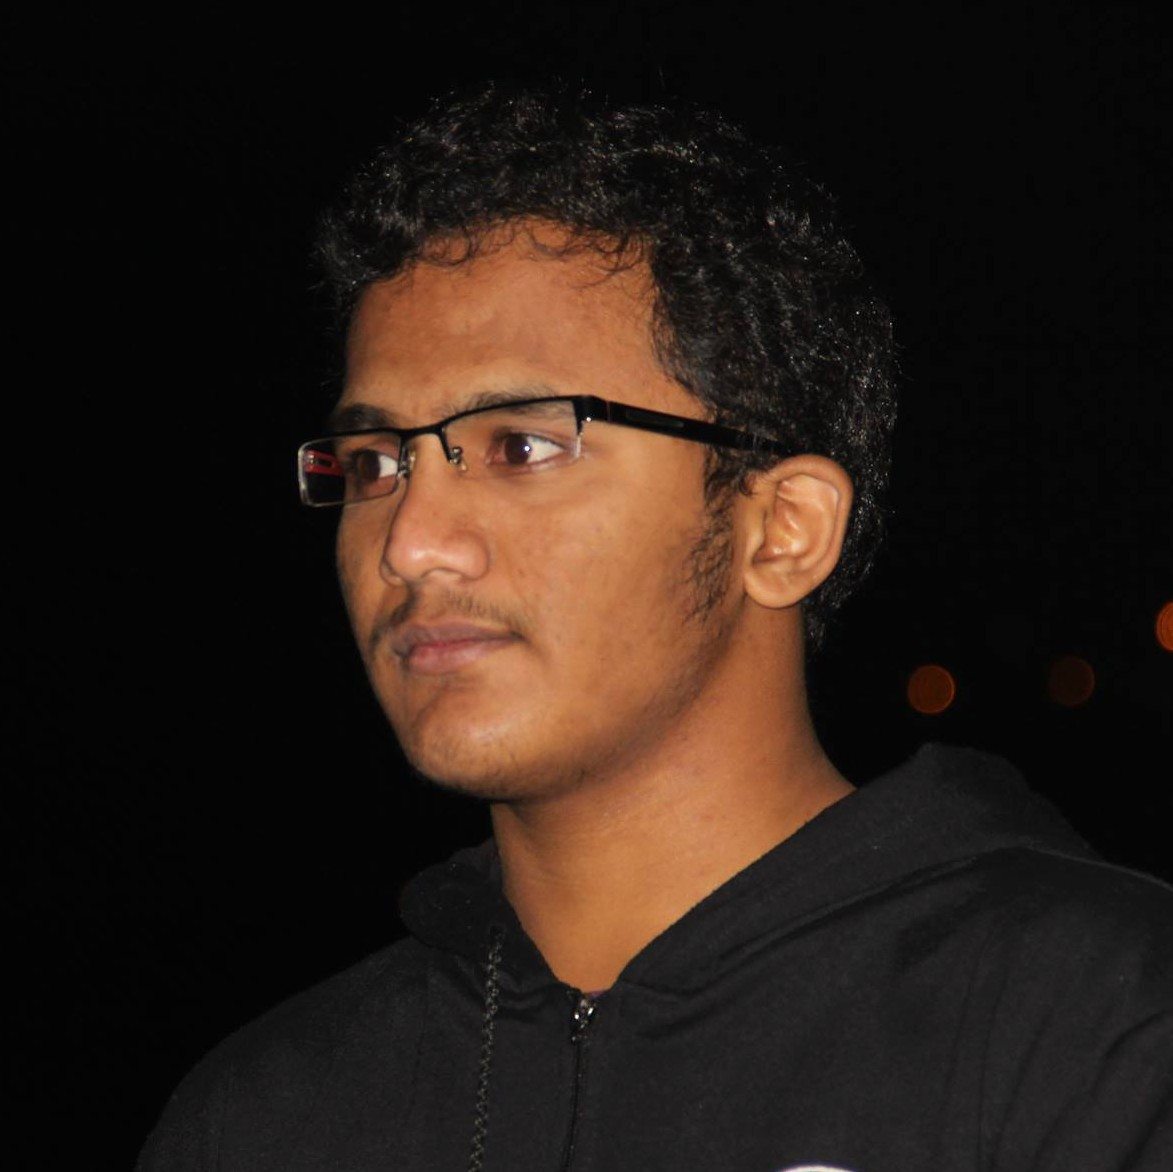
\includegraphics[width=0.25\textwidth]{photo.jpg}
\end{wrapfigure}
%................................................end..................................................................%

%..............................................Personal Details.........................................................%
\MyName{Manikanta Reddy D}
\begin{flushright}
	$2^{nd}$ year undergraduate\\
	Dept. of Computer Sciences\\
	Indian Institue of Technology, Kanpur
\end{flushright}
%..............................................end......................................................................%

\sepspace

%..........................................EDU INFO....................................................................%
\NewPart{Education}{}

\EducationEntry{B.Tech, Computer Sciences}{2013-}{Indian Institute of Technology, Kanpur}{8.0/10.0}

\sepspace

\EducationEntry{Intermediate}{2011-2013}{Sri Chaitanya Narayana Group, Hyderabad}{96.9/100}

\sepspace

\EducationEntry{High School}{2000-2011}{Sri Chaitanya Group, Hyderabad}{94.3/100}

%............................................end............................................................%

%......................................ACH ZONE.............................................................%
\NewPart{Scholastic Acheivements}{}

\ScholasticAcheivements{AIR 121}{Gold Medal}{IIT-JEE, 2013}{IGNOU-SAARC Olympiad, 2011}

\sepspace

\ScholasticAcheivements{KVPY Scholar}{Aditya Birla Scholarship}{Placed 37th in CML, 2011}{Nominated in 2013}
%.............................................end.......................................................%
%................................................Skills.................................................%
\NewPart{Skill Set}
	\begin{tabular}{m{0.33\textwidth}  m{0.33\textwidth} m{0.33\textwidth}}
		\SkillsEntry{\textbf{Programming}}{\textbf{Design}}{\textbf{Misc}}
		\SkillsEntry{C}{Photoshop}{R}
		\SkillsEntry{Python}{After Effects}{Weka}
		\SkillsEntry{HTML}{Gimp}{OpenCV}
		\SkillsEntry{CSS}{Blender}{bootstrap}
		\SkillsEntry{js}{Openshot}{reveal.js}
		\SkillsEntry{shell}{}{}
	\end{tabular}
%.................................................end....................................................%
%.......................................Projects......................................................%
\NewPart{Projects}

\WorkEntry{Gesture\,Recognition}{May-Jul 2014}{$\bullet$ Developed an Application in C using \emph{OpenCV} capable of recognising gestures made by us.\\ $\bullet$ The video input was fed into the system which then characterised the motion of the hand into characteristic
directions after passing various Gaussian filters and thereby used them to understand the gesture and
hence execute a gesture.\\$\bullet$We then approched an other method of Gesture recognition using HSV color spaces and thresholdings}
\sepspace

\WorkEntry{Analysis of Gamma Ray Data from Markarian 421 and Crab}{Dec 2013}{$\bullet$This project involved Analysing Data from Gamma Ray Telescopes under Dr. K.K Yadav and Dr. R. C Rannot,
at BARC, Mumbai.\\$\bullet$The processing of images, made available from various cherenkov detectors, involved developing algorithms
for separating objects by identifying boundaries/ edges in the low resolutions images}
\sepspace
\WorkEntry{Carnival of Rust}{Aug-Nov\,2014}{$\bullet$A project by our Team was adjudged to be the Best Sectional Project in the course TA201\\$\bullet$The project involved modelling an \emph{amusement park} utilising many industrial processes varying from \emph{casting, welding, shearing,} etc.}

%.............................................end........................................................%

%..............................................POR

%.......................................TRANSCRIPT ZONE.................................................%
\begin{center}
	\tiny{INDIAN INSTITUTE OF TECHNOLOGY}\\
	\tiny{GRADE REPORT}\\
	\tiny{ROLL NO : 13265} \hfill \tiny{DEPARTMENT : COMPUTER SC. \& ENGG.}\\
	\tiny{NAME : DORNALA MANIKANTA REDDY} \hfill \tiny{PROGRAM : BACHELOR OF TECHNOLOGY}\\
\end{center}
\begin{center}
	\begin{tabular}{m{5em}  m{1.5cm} m{5cm} m{0.5cm} m{0.7cm} m{0.3cm} m{0.5cm}} 
	\hdashline
	\tiny{\textbf{YEAR/SEM}} & \transcriptentry{\textbf{COURSE}}{\textbf{TITLE}}{\textbf{UNIT}}{\textbf{GRADE}}{\textbf{SPI}}{\textbf{CPI}}
	\hdashline
	\multirow{7}{5em}{\tiny{2013-2014 FIRST}}
		& \transcriptentry{CHM101A}{CHEMISTRY\,LABORATORY}{3}{A}{}{}
		& \transcriptentry{ESC101A}{FUNDAMENTALS\,OF\,COMPUTING}{14}{B}{}{}
		& \transcriptentry{MTH101A}{MATHEMATICS\,I}{11}{B}{}{}
		& \transcriptentry{PE101A}{MORNING\,EXERCISE}{3}{S}{}{}
		& \transcriptentry{PHY103A}{PHYSICS\,II}{11}{C}{}{}
		& \transcriptentry{PSY151A}{INTRODUCTION\,TO\,PSYCHOLOGY}{11}{B}{}{}
		& \transcriptentry{}{}{}{}{7.7}{7.7}
		\\
	\multirow{7}{5em}{\tiny{2013-2014 SECOND}}
		& \transcriptentry{CHM102A}{GENERAL\,CHEMISTRY}{8}{B}{}{}
		& \transcriptentry{LIF101A}{INTRODUCTION\,TO\,BIOLOGY}{6}{B}{}{}
		& \transcriptentry{MTH102A}{MATHEMATICS\,II}{11}{B}{}{}
		& \transcriptentry{PE102A}{EVENING\,EXERCISE}{3}{S}{}{}
		& \transcriptentry{PHY101A}{PHYSICS\,LABORATORY}{3}{B}{}{}
		& \transcriptentry{PHY102A}{PHYSICS\,I}{11}{A}{}{}
		& \transcriptentry{TA101A}{ENGINEERING\,GRAPHICS}{9}{A}{}{}
		& \transcriptentry{}{}{}{}{8.8}{8.2}
		\\	
	\multirow{7}{5em}{\tiny{2014-2015 FIRST}}
		& \transcriptentry{COM200}{COMMUNICATIONS\,SKILLS:\,COMPOSITION}{5}{S}{}{}
		& \transcriptentry{CS201A}{MATHEMATICS\,FOR\,COMPUTER\,SCIENCE-I}{9}{C}{}{}
		& \transcriptentry{CS210A}{DATA\,STRUCTURES\,AND\,ALGORITHMS}{12}{B}{}{}
		& \transcriptentry{ESC201A}{INTRODUCTION\,TO\,ELECTRONICS}{14}{B}{}{}
		& \transcriptentry{ES0202A}{MECHANICS\,OF\,SOLIDS}{11}{B}{}{}
		& \transcriptentry{TA201A}{MANUFACTURING\,PROCESSES\,I}{6}{B}{}{}
		& \transcriptentry{}{}{}{}{7.7}{8.0}\\
	\hdashline
	\end{tabular}
\end{center}
%........................................end................................................................%

\end{document}